\item Plot the given functions and find their Fourier Transforms
%
\begin{enumerate}
  \item
  $\displaystyle
  f(x) =
  \begin{cases}
    -1 & \text{if } -1 < x < 0\\
    1 &  \text{if } 0 < x < 1\\
    0 & \text{otherwise}
  \end{cases}
  $
  \item
  $\displaystyle
  f(x) =
  \begin{cases}
    1 - |x| & \text{if } |x| \leq 1\\
    0 & \text{otherwise}
  \end{cases}
  $
\end{enumerate}

\bigbreak

Here, let us consider both problems individually.

\begin{enumerate}
  \item First, let us consider our first given equation:

  $\displaystyle
  f(x) =
  \begin{cases}
    -1 & \text{if } -1 < x < 0\\
    1 &  \text{if } 0 < x < 1\\
    0 & \text{otherwise}
  \end{cases}
  $

  Here, let us plot our given function:

  \begin{center}
    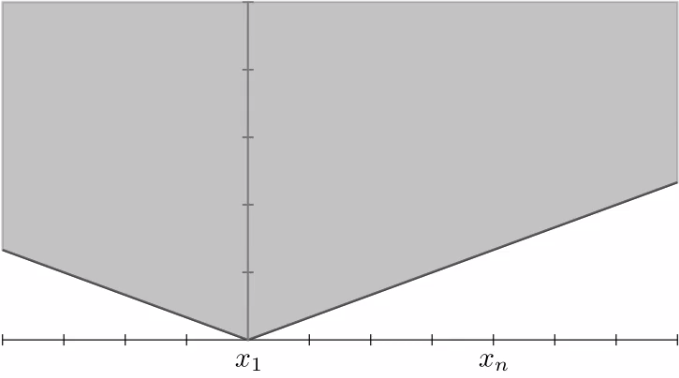
\includegraphics[height=8cm]{2a}
  \end{center}

  Now, let us find the Fourier Transform of this problem.

  Here, let us consider our domain of integration, where $f_i$ is the $i^{\text{th}}$ position. Let us informally write:
  %
  \begin{align}
    f_1(x) & = \int^0_{-1} -1 \text{ dx}\\
    f_2(x) & = \int^1_0 1 \text{ dx}\\
    f_3(x) & = \int^{-1}_{-\infty} 0 \text{ dx} + \int^\infty_1 0 \text{ dx}
  \end{align}

Here, let us write our definition of the Fourier Transform:
%
\begin{align}
  F[f] & = \frac{1}{\sqrt{2 \pi}} \int^\infty_{-\infty} f(x) e^{-i \xi x} \text{ dx}
\end{align}

From here, let us split our integral:
%
\begin{align}
  F[f]
  % Initial Definition
  & =
  \frac{1}{\sqrt{2 \pi}}
  \left[
    \int^0_{-1} -           e^{-i \xi x}  \text{ dx}
  + \int^1_0                e^{-i \xi x}  \text{ dx}
  + \int^{-1}_{- \infty}  0 e^{-i \xi x}  \text{ dx}
  + \int^\infty_1         0 e^{-i \xi x}  \text{ dx}
  \right]\\
  % Remove 0's
  & =
  \frac{1}{\sqrt{2 \pi}}
  \left[
  - \int^0_{-1} e^{-i \xi x} \text{ dx}
  + \int^1_0    e^{-i \xi x} \text{ dx}
  \right]
\end{align}

Here, let us integrate our integrals:
%
\begin{align}
  F[f]
  % Initial
  & =
  \frac{1}{\sqrt{2 \pi}}
  \left[
  - \int^0_{-1} e^{-i \xi x} \text{ dx}
  + \int^1_0    e^{-i \xi x} \text{ dx}
  \right]\\
  % Integrate
  & =
  \frac{1}{\sqrt{2 \pi}}
  \left[
  - \frac{1}{-i \xi} e^{-i \xi x} \Big|^0_{-1}
  + \frac{1}{-i \xi} e^{-i \xi x} \Big|^1_0
  \right]\\
  % Move values out
  & =
  \frac{1}{i \xi \sqrt{2 \pi}}
  \left[
    e^{-i \xi x} \Big|^0_{-1}
  - e^{-i \xi x} \Big|^1_0
  \right]\\
  % Evaluate
  & =
  \frac{1}{i \xi \sqrt{2 \pi}}
  \left[
  \left(
  e^{-i \xi 0} - e^{-i \xi (-1)}
  \right)
  -
  \left(
  e^{-i \xi 1} - e^{-i \xi 0}
  \right)
  \right]\\
\end{align}

Here, let us evaluate our expressions and simplify:
%
\begin{align}
  & =
  \frac{1}{i \xi \sqrt{2 \pi}}
  \left[
  \left(
  1 - e^{i \xi}
  \right)
  -
  \left(
  e^{-i \xi} - 1
  \right)
  \right]\\
  % Distribute
  & =
  \frac{1}{i \xi \sqrt{2 \pi}}
  \left[
  1 - e^{i \xi}
  - e^{-i \xi} + 1
  \right]\\
  % Distribute
  & =
  \frac{2}{i \xi \sqrt{2} \sqrt{\pi}}
  \left[
  - e^{i \xi} - e^{-i \xi}
  \right]\\
  % Setup for substitution
  & =
  \frac{\sqrt 2}{\xi \sqrt \pi}
  \frac{e^{i \xi} + e^{-i \xi}}{i}\\
  & =
  \frac{\sqrt 2}{\xi \sqrt \pi}
  \frac{2 \cos(\xi)}{i}
\end{align}


%______________________________________________________________________________%
\setcounter{equation}{0}
\newpage
\item Now, let us consider our second given equation:

$\displaystyle
f(x) =
\begin{cases}
  1 - |x| & \text{if } |x| \leq 1\\
  0 & \text{otherwise}
\end{cases}
$

Here, let us plot our given function:

\begin{center}
  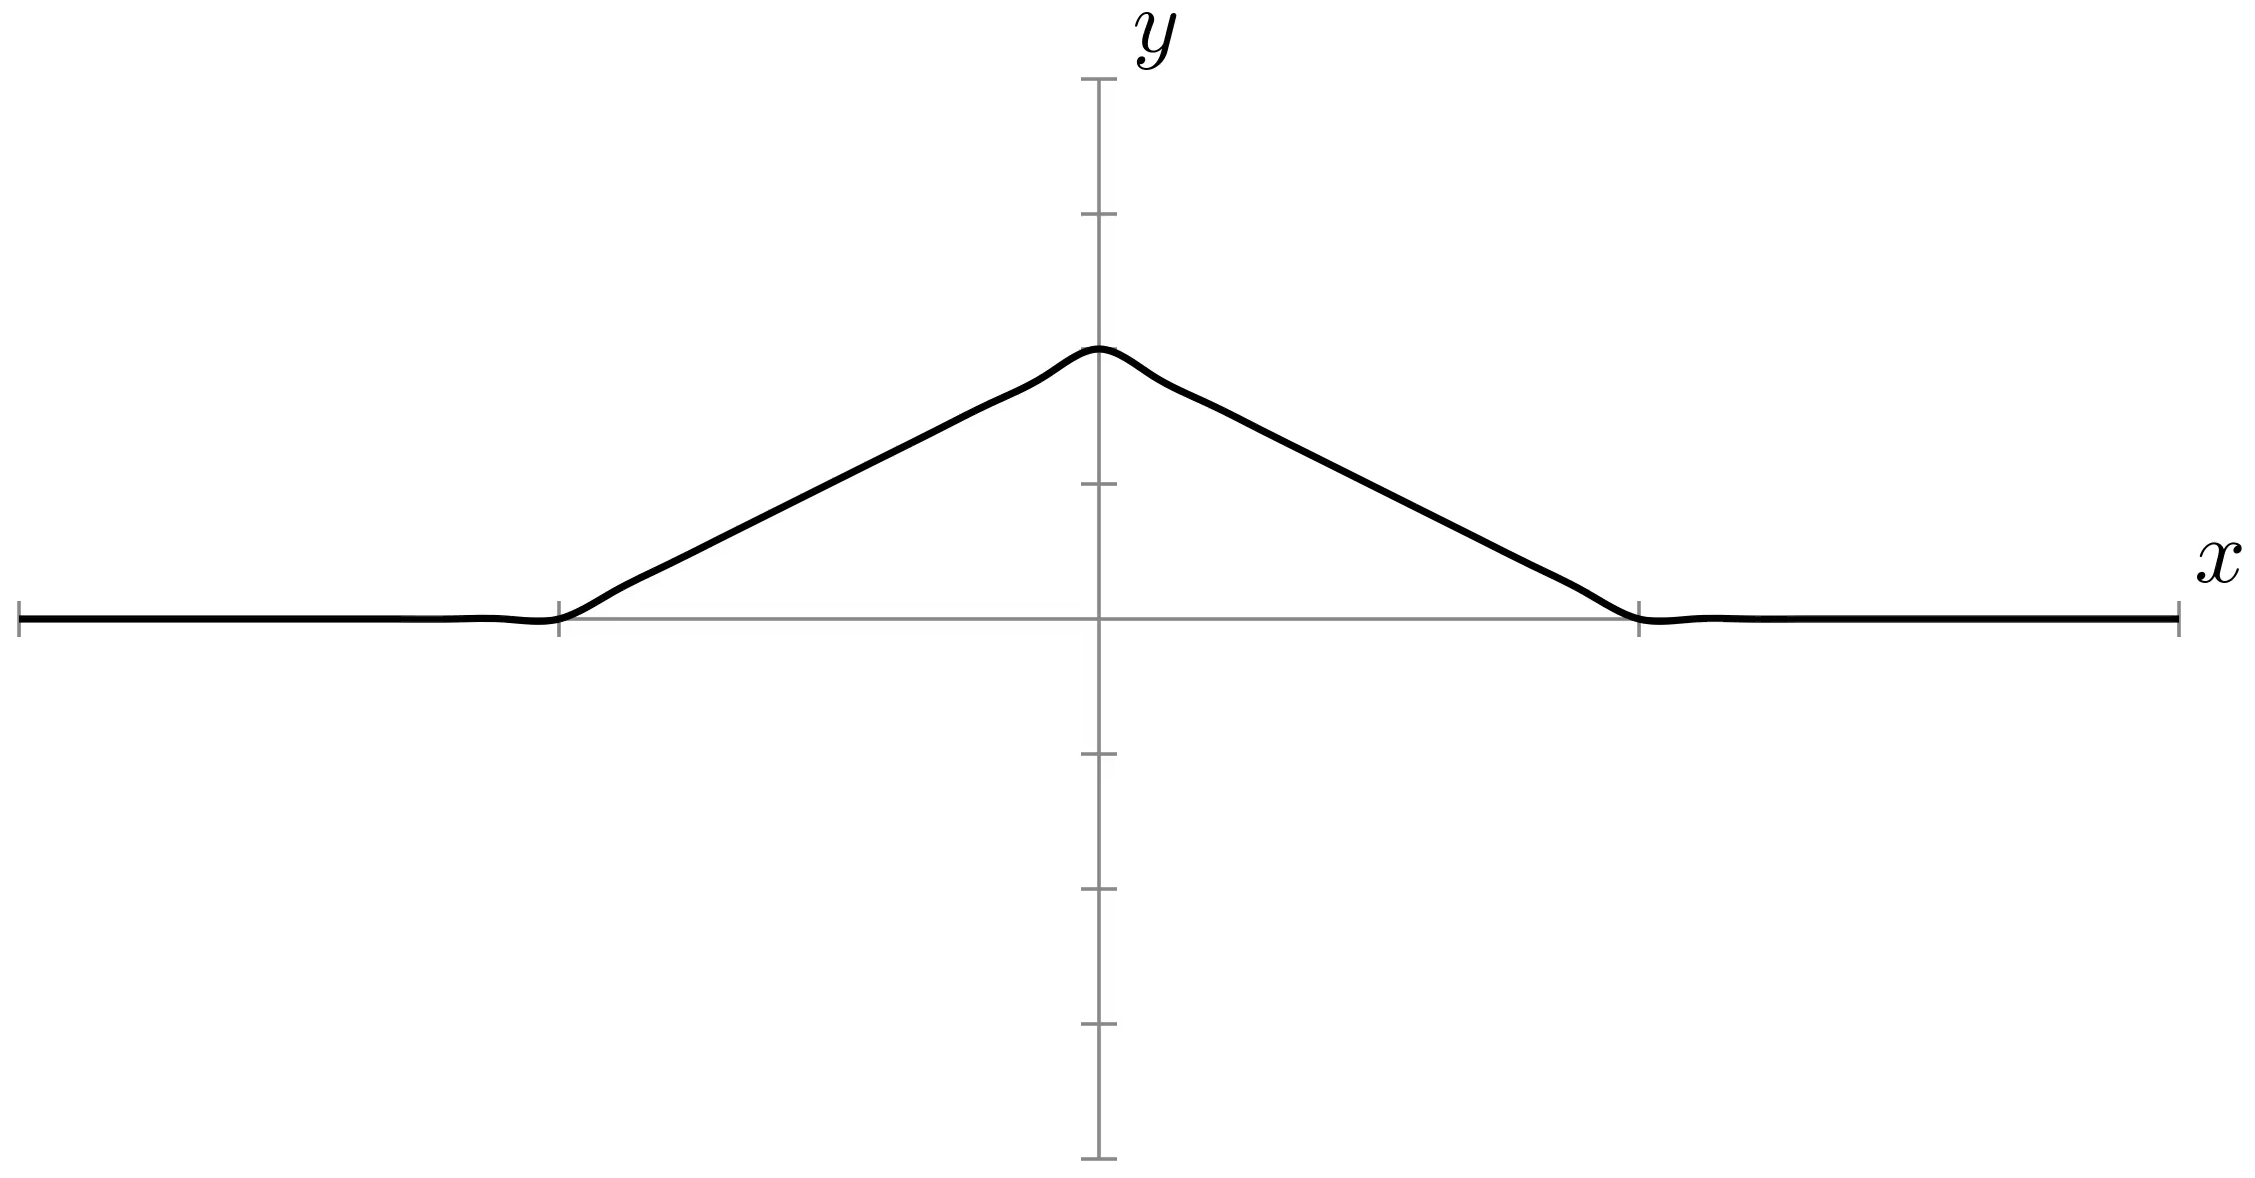
\includegraphics[height=8cm]{2b}
\end{center}

Now, let us find the Fourier Transform of this problem.

Here, let us write our equation and further divide our function:
%
\begin{align}
  f_1(x) & = \int^1_0 1 - x \text{ dx}\\
  f_2(x) & = \int^0_{-1} 1 + x \text{ dx}\\
  f_3(x) & = \int^\infty_1 0 \text{ dx } + \int^{-1}_{-\infty} 0 \text{ dx}
\end{align}

Here, let us use the definition of the Fourier Transform from 4) is the previous part. First, let us split our integral:
%
\begin{align}
  F[f]
  % Initialize
  & = \frac{1}{\sqrt{2 \pi}}
  \left[
    \int^1_0            (1 - x) e^{-i \xi x} \text{ dx}
  + \int^0_{-1}         (1 + x) e^{-i \xi x} \text{ dx}
  + \int^\infty_1       0     e^{-i \xi x} \text{ dx }
  + \int^{-1}_{-\infty} 0     e^{-i \xi x} \text{ dx}
  \right]\\
  % Simplify
  & =
  \frac{1}{\sqrt{2 \pi}}
  \left[
    \int^1_0    (1 - x) e^{-i \xi x} \text{ dx}
  + \int^0_{-1} (1 + x) e^{-i \xi x} \text{ dx}
  \right]\\
  % Distribute
  & =
  \frac{1}{\sqrt{2 \pi}}
  \left[
    \int^1_0    e^{-i \xi x} - x e^{-i \xi x} \text{ dx}
  + \int^0_{-1} e^{-i \xi x} + x e^{-i \xi x} \text{ dx}
  \right]
\end{align}

Before proceeding, let us create a table of integration:

\begin{center}
  \begin{tabular}{c|c}
    $x$ &  $                    e^{-i \xi x}$\\
    \hline
    $1$ &  $\frac{1}{-i \xi}    e^{-i \xi x}$\\
    \hline
    $0$ &  $\frac{1}{i^2 \xi^2} e^{-i \xi x}$
  \end{tabular}
\end{center}

Here, we have our integration by parts. Now, let us proceed with our integrals:
%
\begin{align}
  F[f]
  % Integrate
  & =
  \frac{1}{\sqrt{2 \pi}}
  \left[
    \left[
       \left(\frac{1}{-i \xi} e^{-i \xi x}\right)
     - \left(\frac{x}{- i \xi} e^{-i \xi x} + \frac{1}{\xi^2} e^{-i \xi x}\right)
    \right]^1_0
  + \left[
      \left(\frac{1}{-i \xi} e^{-i \xi x}\right)
    + \left(\frac{x}{- i \xi} e^{-i \xi x} + \frac{1}{\xi^2} e^{-i \xi x}\right)
    \right]^0_{-1}
  \right]\\
  % Simplify
  & =
  \frac{1}{\sqrt{2 \pi}}
  \left[
    \left[
     - \frac{1}{ i \xi} e^{-i \xi x}
     + \frac{x}{ i \xi} e^{-i \xi x}
     - \frac{1}{ \xi^2} e^{-i \xi x}
    \right]^1_0
  + \left[
    - \frac{1}{ i \xi} e^{-i \xi x}
    - \frac{x}{ i \xi} e^{-i \xi x}
    + \frac{1}{ \xi^2} e^{-i \xi x}
    \right]^0_{-1}
  \right]
\end{align}

Here, let us evaluate both integrals side-by-side:
\bigbreak
\begin{multicols}{2}
  Let us consider the integral on the left:
\begin{align}
  &
  \left[
    - \frac{1}{ i \xi} e^{-i \xi x}
    + \frac{x}{ i \xi} e^{-i \xi x}
    - \frac{1}{ \xi^2} e^{-i \xi x}
  \right]^1_0\\
  % Plug in
  &
  % 1 side
  \left(
    - \frac{1}{ i \xi} e^{-i \xi}
    + \frac{1}{ i \xi} e^{-i \xi}
    - \frac{1}{ \xi^2} e^{-i \xi}
  \right)
  % 0 side
  +
  \left(
    \frac{1}{ i \xi}
  + \frac{1}{ \xi^2}
  \right)
\end{align}
  Now, let us consider the integral on the right:
\begin{align}
  &
  \left[
  - \frac{1}{ i \xi} e^{-i \xi x}
  - \frac{x}{ i \xi} e^{-i \xi x}
  + \frac{1}{ \xi^2} e^{-i \xi x}
  \right]^0_{-1}\\
  % Plug in
  &
  % 0 side
  \left(
  - \frac{1}{ i \xi}
  + \frac{1}{ \xi^2}
  \right)
  % -1 Side
  +
  \left(
    \frac{1}{ i \xi} e^{i \xi}
  - \frac{1}{ i \xi} e^{i \xi}
  - \frac{1}{ \xi^2} e^{i \xi}
  \right)
\end{align}
\end{multicols}

Now, let us plug in our parts back into our integral:
%
\begin{align}
  F[f]
  & =
  \frac{1}{\sqrt{2 \pi}}
  \left[
    % 1 side
    \left(
      - \frac{1}{ i \xi} e^{-i \xi}
      + \frac{1}{ i \xi} e^{-i \xi}
      - \frac{1}{ \xi^2} e^{-i \xi}
    \right)
    % 0 side
    +
    \left(
      \frac{1}{ i \xi}
    + \frac{1}{ \xi^2}
    \right)
    +
    \left(
    - \frac{1}{ i \xi}
    + \frac{1}{ \xi^2}
    \right)
    % -1 Side
    +
    \left(
      \frac{1}{ i \xi} e^{i \xi}
    - \frac{1}{ i \xi} e^{i \xi}
    - \frac{1}{ \xi^2} e^{i \xi}
    \right)
  \right]\\
  % Step two: Shift
  & =
  \frac{1}{\sqrt{2 \pi}}
  \left[
  \left(
    - \frac{1}{ i \xi} e^{-i \xi}
    + \frac{1}{ i \xi} e^{-i \xi}
    - \frac{1}{ \xi^2} e^{-i \xi}
  \right)
  +
  \left(
  \frac{1}{ i \xi} e^{i \xi}
  - \frac{1}{ i \xi} e^{i \xi}
  - \frac{1}{ \xi^2} e^{i \xi}
  \right)
  +
  \left(
    \frac{1}{ i \xi}
  + \frac{1}{ \xi^2}
  \right)
  +
  \left(
  - \frac{1}{ i \xi}
  + \frac{1}{ \xi^2}
  \right)
  \right]\\
  % Step three: Combine
  & =
  \frac{1}{\sqrt{2 \pi}}
  \left[
  \left(
    - \frac{1}{ \xi^2} e^{-i \xi}
  \right)
  +
  \left(
    - \frac{1}{ \xi^2} e^{i \xi}
  \right)
  +
  \left(
    \frac{1}{ i \xi}
  + \frac{1}{ \xi^2}
  \right)
  +
  \left(
  - \frac{1}{ i \xi}
  + \frac{1}{ \xi^2}
  \right)
  \right]
\end{align}

From here, let us shift our terms around then group them.
%
\begin{align}
  % Step Four: Shift
  & =
  \frac{1}{\sqrt{2 \pi}}
  \left[
  \left(
    - \frac{1}{ \xi^2} e^{-i \xi}
  \right)
  +
  \left(
    - \frac{1}{ \xi^2} e^{i \xi}
  \right)
  +
  \left(
    \frac{1}{ i \xi}
  + \frac{1}{ \xi^2}
  \right)
  +
  \left(
  - \frac{1}{ i \xi}
  + \frac{1}{ \xi^2}
  \right)
  \right]\\
  % Step Five: Group
  & =
  \frac{1}{\sqrt{2 \pi}}
  \left[
  \left(
    - \frac{1}{ \xi^2} e^{-i \xi}
    - \frac{1}{ \xi^2} e^{i \xi}
  \right)
  +
  \left(
   \frac{2}{ \xi^2}
  \right)
  \right]
\end{align}

From here, let us rewrite our exponential and factor our terms.
%
\begin{align}
  & =
  -\frac{1}{\sqrt{2 \pi} \xi^2}
  \left(
      e^{-i \xi}
    + e^{i \xi}
  \right)
  +
   \frac{2}{\sqrt{2 \pi} \xi^2}\\
   %
   & =
   -\frac{\sqrt 2}{\sqrt{\pi} \xi^2} \cos(\xi)
   +
    \frac{\sqrt 2}{\sqrt{\pi} \xi^2}\\
  %
  & =
  -\frac{\sqrt 2}{\sqrt \pi \xi^2} (\cos(\xi) + 1)
\end{align}
\end{enumerate}
